% Chapter Help

\chapter{Theoretical Background} % Main chapter title

\label{Chapter3} % For referencing the chapter elsewhere, use \ref{Chapter1} 

\section{Higgs Production and Decays}
Having discussed the measurement conditions, a brief overview of the underlying theory of the CP measurement is going to be given.\\
There are mainly four Higgs-production mechanisms, which are pictured in Fig. \ref{fig:Higgs_productions}. In this thesis, production and decay mechanisms are also going to be called channels in the following.
\begin{comment}
	\begin{figure}[h]
		\centering
		\feynmandiagram [horizontal=a to b] {
			i1 -- [fermion] a -- [fermion] i2,
			a -- [photon,edge label=\gamma] b,
			f1 -- [fermion] b -- [fermion] f2,
		};
		\feynmandiagram [horizontal=a to b] {
			i1 [particle=\(\pi^{0}\)] -- [fermion] a -- [fermion] i2,
			a -- [dashed] b,
			f1 -- [fermion] b -- [fermion] f2,
		};
	\end{figure}\\
	\begin{figure}[h]
		\centering
		\feynmandiagram [horizontal=a to b] {
			i1 -- [fermion] a -- [fermion] i2,
			a -- [photon,edge label=\gamma] b,
			f1 -- [fermion] b -- [fermion] f2,
		};
		\feynmandiagram [horizontal=a to b] {
		i1 [particle=\(\pi^{0}\)] -- [fermion] a -- [fermion] i2,
		a -- [dashed] b,
		f1 -- [fermion] b -- [fermion] f2,
		};
		\caption{Feynman Diagrams}
		\label{fig:Higgs_productions}
	\end{figure}\\
\end{comment}
\begin{figure}[h]
	\centering
	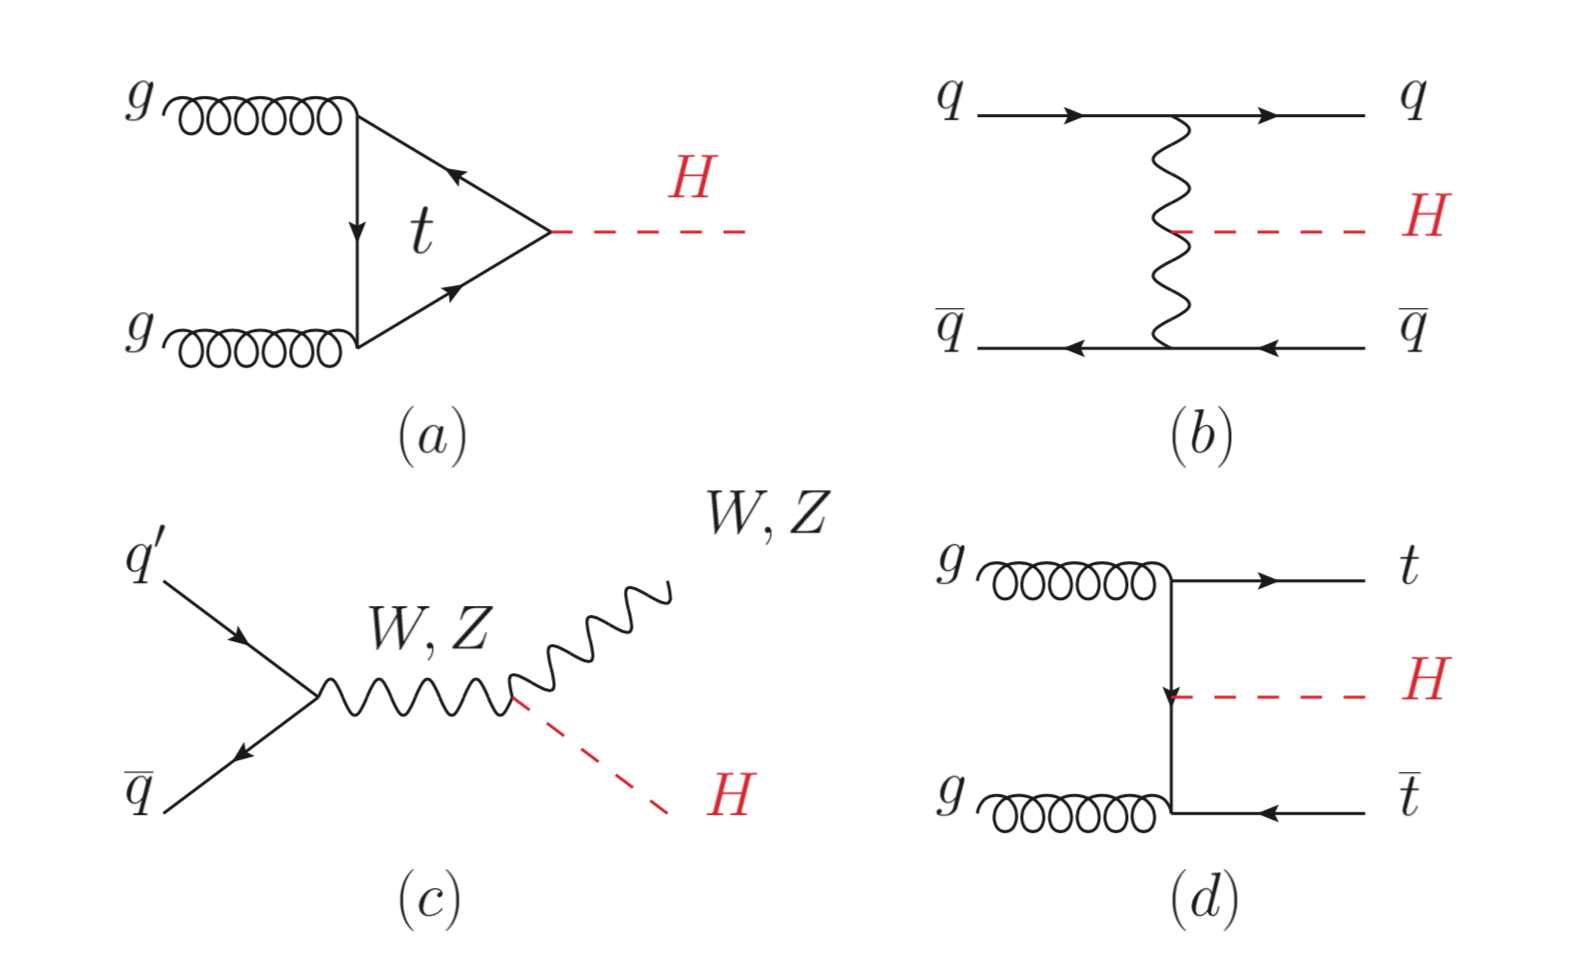
\includegraphics[width=0.7\linewidth]{Figures/Higgs-production_PDG_Huge_p183}
	\caption{Feynman Diagrams of different Higgs production channels. Source: \parencite{PDG_source}}
	\label{fig:Higgs_productions}
\end{figure}\\
During the first and most common production mechanism -- the so-called gluon-gluon fusion or ggH -- two gluons fuse through a top-loop into an $H$, since they do not couple to the Higgs boson directly as massless particles. The second most common channel is the vector boson fusion (VBF) where two quarks radiate a $Z$ or $W$ boson, which then produce an $H$. In the third case called Higgsstrahlung, a Higgs boson is radiated by a $W$ or $Z$ produced by a fusion of an quark-antiquark pair. During the fourth and least common channel, a pair of top (or bottom) quarks are also produced as "by-products". \\
As mentioned in the Introduction Ch.\ref{Chapter1}, one has already measured the parity of the Higgs boson in its diboson decay channel, yielding a CP-even state being consistent with the SM prediction. Nevertheless, studying the ditau decay channel, a new term emerges in the Lagrangian of the system, which gives rise to a possible mixing between CP-odd and CP-even states. In Fig. \ref{fig:Higgs_decays}, several decay mechanisms are listed, among which the $b\overline{b}$ event seems to be the most accessible. However, there are several limitations measuring the bottom quark polarisation. For this reason, the ditau channel is going to be favoured in this thesis.
\begin{figure}[h]
	\centering
	\subfigure{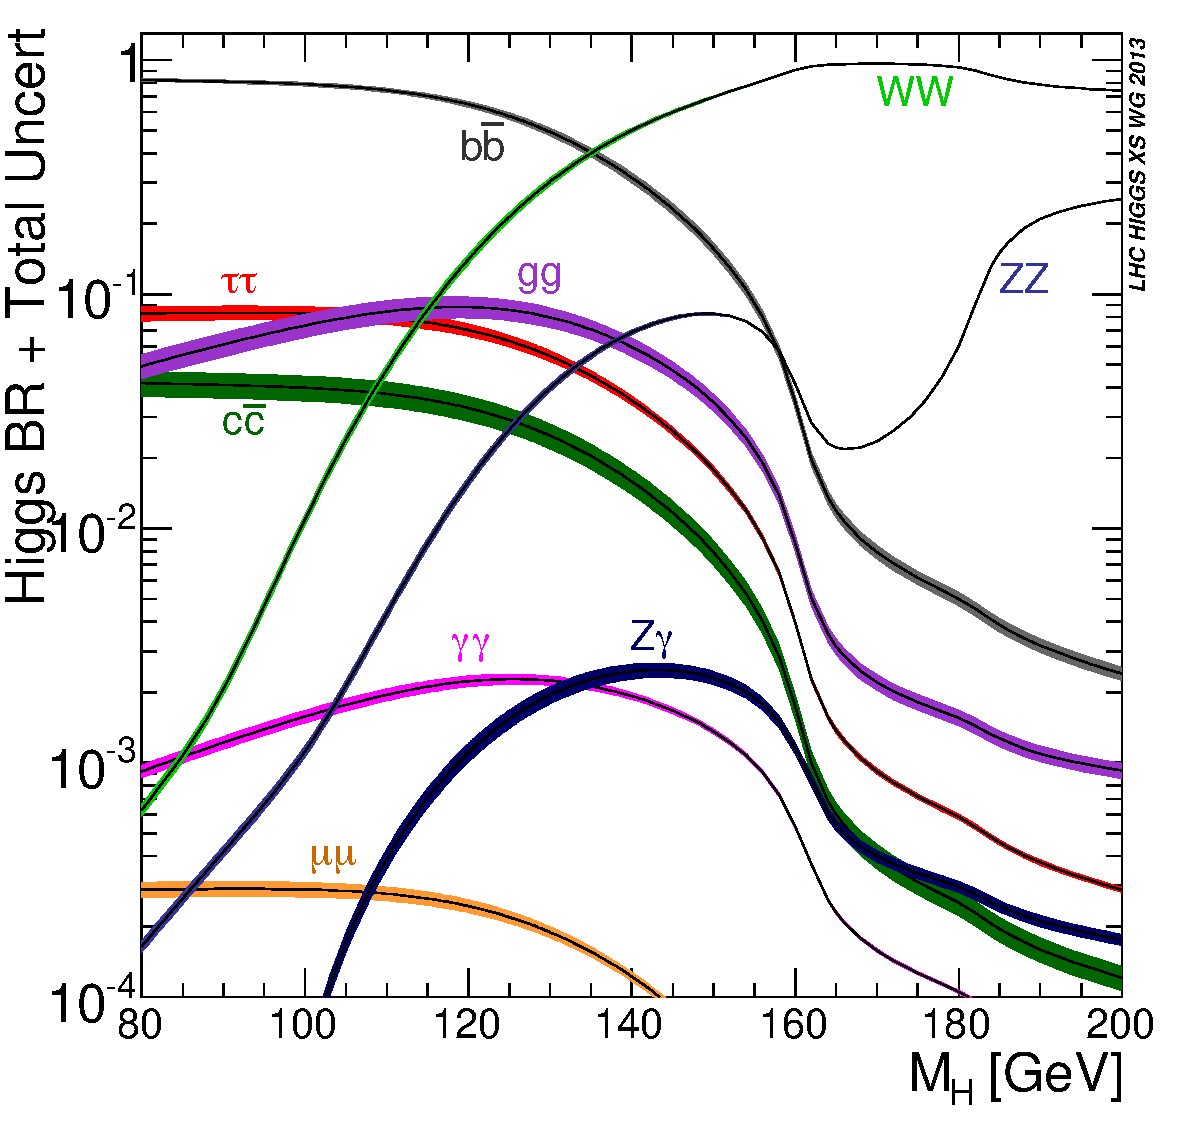
\includegraphics[width=0.4\linewidth]{Figures/Higgs_BR_LM_eps.pdf}}	\subfigure{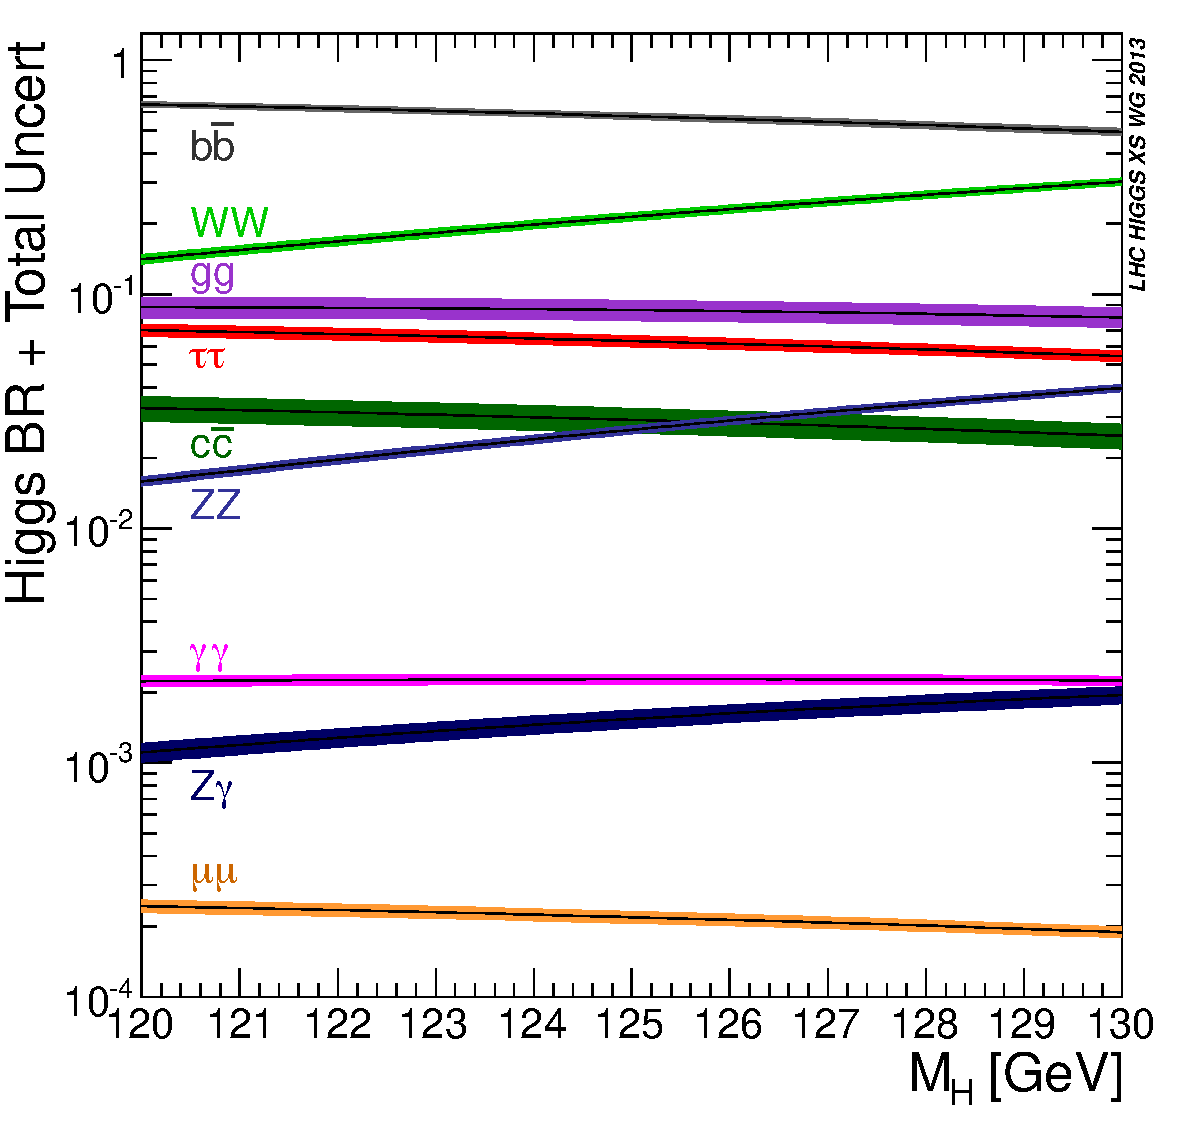
\includegraphics[width=0.4\linewidth]{Figures/Higgs_BR_120-130_eps.pdf}}
	\caption{Left: The branching ratios (BR) of Higgs decays for several theoretical Higgs masses\\Right: The decay BRs in the $m_H = 125$ GeV region}
	\label{fig:Higgs_decays}
\end{figure}
\section{The CP-Mixing}
In order to proceed, one should also introduce the charge conjugation operator $\hat{C}$ and the parity operator $\hat{P}$. \\
The parity operator is defined by the transformation $\hat{P}: \mathbb{R}^3 \rightarrow \mathbb{R}^3, \, \boldsymbol{x} \mapsto -\boldsymbol{x}$; i.e. it corresponds to a point reflection with respect to the origin. The charge conjugation $\hat{C}$ operator assigns each particle its antiparticle, e.g. for a lepton $l$, $\hat{C}\ket{l} = \ket*{\overline{l}}$ holds. The combination of the two operators yields the $\hat{C}\hat{P}$-operator, which has two eigenvalues $\lambda_\pm=\pm 1$, where $\lambda_+=+1$ is called CP-even and $\lambda_-=-1$ is called CP-odd eigenstate. One can also show that a normalised superposition of a CP-even and a CP-odd eigenstate $\ket{e}$ and $\ket{o}$ is not an eigenstate of the $\hat{C}\hat{P}$-operator anymore:
\begin{equation}
	\hat{C}\hat{P} \left(\sin\alpha\ket{e}+\cos\alpha\ket{o}\right) = \sin\alpha\ket{e}-\cos\alpha\ket{o} \neq \sin\alpha\ket{e}+\cos\alpha\ket{o}
\end{equation}
Now consider the Lagrangian $\mathcal{L}$ of the ditau decay channel \parencite{Berge_DY_bckg}, which is described by the Yukawa Langrangian $\mathcal{L}_Y$:
\begin{equation}
	\mathcal{L}_Y = -\left(\sqrt{2} G_F\right)^\frac{1}{2} m_\tau (a_\tau \overline{\tau}\tau+b_\tau \overline{\tau}i\gamma_5\tau)h
\end{equation}
where $G_F$ denotes the Fermi-constant and $a_\tau, b_\tau$ are the reduced dimensionless Yukawa coupling constants, $\gamma_5$ is the Dirac-matrix, and $\tau$ and $h$ are the Dirac and scalar field respectively. Rewriting this Lagrangian as
\begin{center}
	\begin{tabular}{ll}
		$\mathcal{L}_Y $ & $= -\underbrace{\left(\sqrt{2} G_F\right)^\frac{1}{2} m_\tau\sqrt{a_\tau^2+b_\tau^2}}_\text{$g_\tau$} \left(\underbrace{\frac{a_\tau}{\sqrt{a_\tau^2+b_\tau^2}}}_\text{$\cos\varphi_\tau$} \overline{\tau}\tau+\underbrace{\frac{b_\tau}{\sqrt{a_\tau^2+b_\tau^2}}}_\text{$\sin\varphi_\tau$} \overline{\tau}i\gamma_5\tau\right)h$\\
		 & $= - g_\tau \left(\cos\varphi_\tau\overline{\tau}\tau+\sin\varphi_\tau\overline{\tau}i\gamma_5\tau\right)h$
	\end{tabular}
\end{center}
with an effective coupling strength $g_\tau$, one can see that $\varphi_\tau$ describes a degree of mixing between the scalar and the pseudoscalar coupling, corresponding to CP-even and CP-odd scenarios. For this reason, $\varphi_\tau$ is going to be denoted as the mixing angle between these two states, and is going to be an object of key importance in this thesis.\\
In case of the measured SM Higgs discussed above the parity was found to be even, corresponding to $\varphi_\tau = 0$. Current ATLAS and CMS measurements \parencite{CMS_CP_odd_exclusion,ATLAS_CP_odd_exclusion} disfavour a pure CP-even scenario, i.e. where $\varphi_\tau = \frac{\pi}{2}$. The main constraint of this measurement in the indirect accessibility of $\varphi_\tau$, so one needs to find and measure an observable, which is related to it.
\section{The IP method}
\label{sec:IP_method}
There are multiple possible final states concerning the taus in the $H\rightarrow\tau\tau$ decay channels which have to be considered separately for this problem. In the following section, this thesis is going to focus on the two-prong ($\tau \rightarrow \pi\pi^0$), one-prong ($\tau \rightarrow \nu_\tau\pi$) and leptonic ($\tau \rightarrow \nu_\tau\overline{\nu}_\mu \mu$) decays, which can be used to construct an observable related to $\varphi_\tau$.\\
It has been shown in \parencite{Berge_1prong, Berge_CP_Prospects} that the angle between the decay planes of the child particles is such an observable. For this, one has to reconstruct these planes, for which depending on the decay channel two methods can be used. In case of a two-prong decay, the 3-momentum of the two pions span a plane, which can be used for the $\varphi_\tau$-study. In case of a leptonic or in a one-prong decay, one could use the surface spanned by the impact parameter vector of the charged child and the direction of its momentum. In order to gain an overview, these cases have been portrayed in Fig. \ref{fig:claudiadecayplanes}.
\begin{figure}[h]
	\centering
	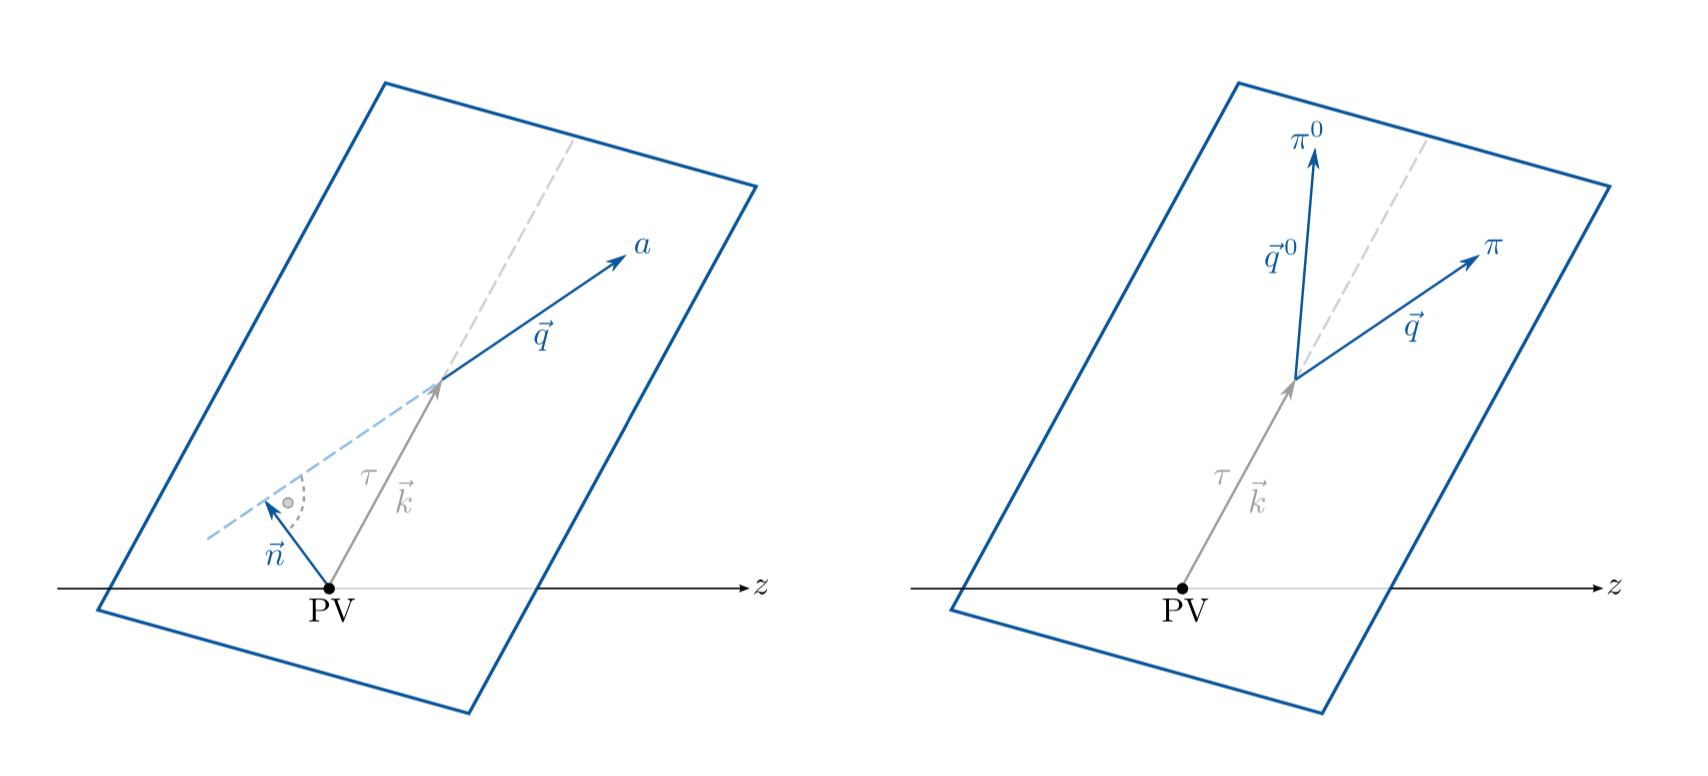
\includegraphics[width=0.7\linewidth]{Figures/Claudia_decay_planes}
	\caption{The channel dependent ways of CP-relevant decay plane reconstruction. Here, the impact parameter vector is denoted by $\protect\overrightarrow{n}$ and momenta by $\protect\overrightarrow{q}$; the vector to the secondary vertex (SV) of $\tau$ decay is called $\protect\overrightarrow{k}$. Source \parencite{Claudia_thesis}}
	\label{fig:claudiadecayplanes}
\end{figure}\\
Concerning the angle between the decay planes $\varphi_{CP}^*$ defined by the child particles of the taus, the following distribution can be found between $\varphi_{CP}^*$ and $\varphi_\tau$ (where the star denotes the zero momentum frame ZMF):
\begin{equation}
	\label{eq:CP_Star_Distribution}
	\frac{d\sigma}{d\varphi_{CP}^*} \sim const - \cos(\varphi_{CP}^*-2\varphi_\tau).
\end{equation}
where $\varphi_{CP}^*$ is defined as
\begin{equation}
	\varphi_{CP}^* = \left\lbrace\begin{array}{cc}
	\varphi^*, \bigskip &\text{if } \mathcal{O_{CP}^*}\geq 0\\
	2\pi-\varphi^*, \bigskip &\text{if } \mathcal{O_{CP}^*}< 0
	\end{array}\right.
\end{equation}
with an $\mathcal{O_{CP}^*}$ and $\varphi^*$ given by
\begin{equation}
	\mathcal{O_{CP}^*} = \boldsymbol{\hat{p}^*}_- \cdot (\boldsymbol{\hat{d}}_-^*\times\boldsymbol{\hat{d}}_+^*).
\end{equation}
Here, $\boldsymbol{\hat{d}_\pm^*}$ are the normalised impact parameter vectors (which are defined by the minimum distance between the straight line defined by the momentum of the child particle and the primary vertex PV) of the $\tau^\pm$ daughter particles in the zero momentum frame (ZMF), and $\boldsymbol{\hat{p}}_-$ is the normalised 3-momentum vector of the negatively charged daughter particle. For two 1-prong decays, these observables have been portrayed in Fig. \ref{fig:decayplanesphistar}.
\begin{figure}[h]
	\centering
	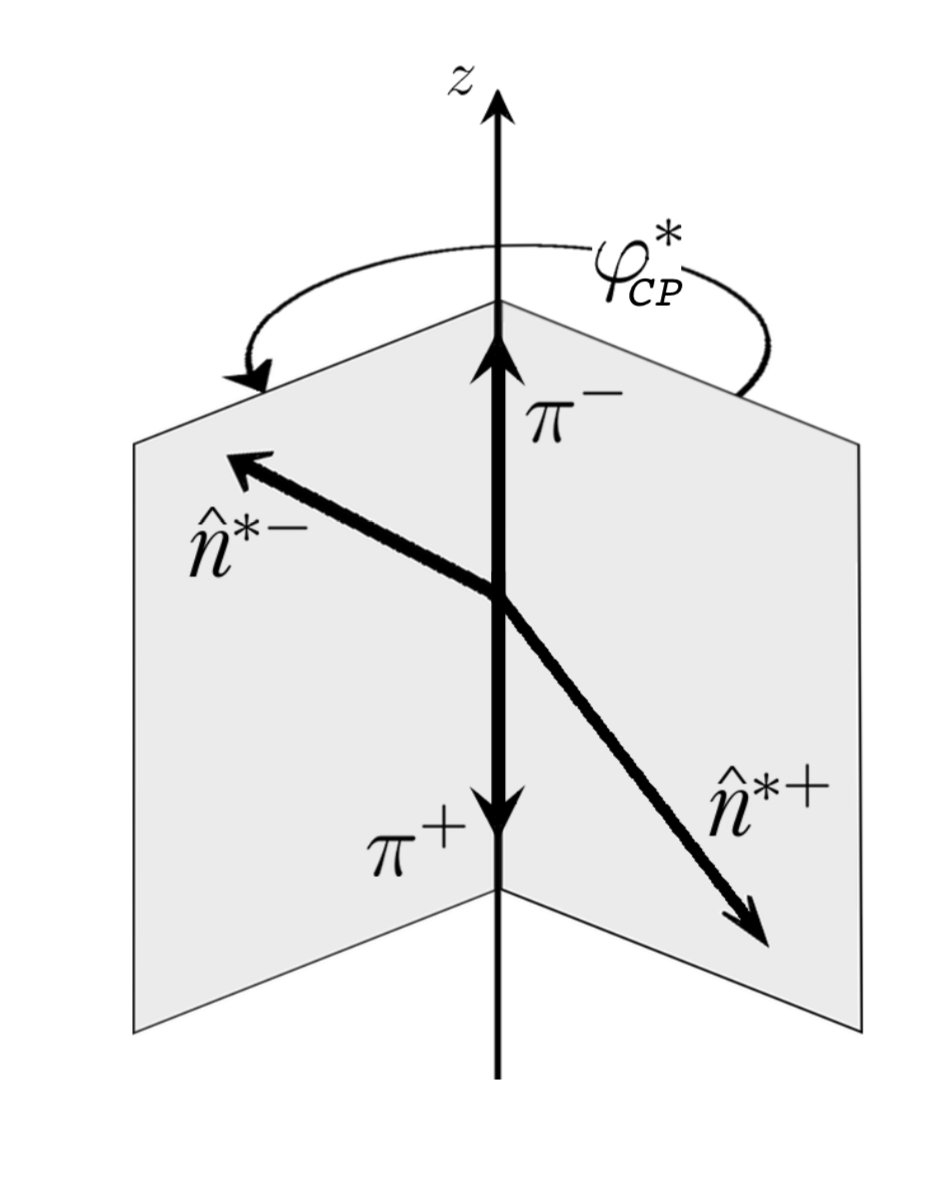
\includegraphics[width=0.3\linewidth]{Figures/decay_planes_phi_Star}
	\caption{The defintion of $\varphi_{CP}^*$. Source: \parencite{Berge_CP_Prospects}}
	\label{fig:decayplanesphistar}
\end{figure}
\begin{figure}[h]
	\centering
	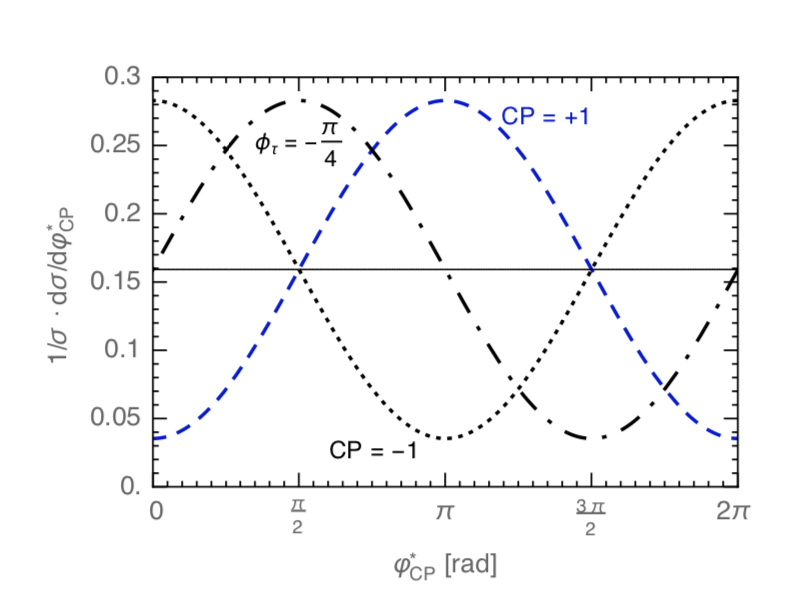
\includegraphics[width=0.5\linewidth]{Figures/Phi_star_distribution}
	\caption{Theoretical $\varphi_{CP}^*$ distributions for different mixing angle scenarios. Source \parencite{Berge_CP_Prospects}}
	\label{fig:phistardistribution}
\end{figure}\\
To summarise: the angle between the decay planes is related to the mixing angle $\varphi_\tau$ through Eq. \ref{eq:CP_Star_Distribution}, such that the reconstruction of these is sufficient to obtain it. For this, in cases of two-prong ($\pi\pi^0$) decays of the $\tau$, one can take the plane spanned by the pions; in cases of the leptonic ($\mu$) or 1-prong ($\pi$) hadronic decay channels, one has to calculate the impact parameter of the child particles to obtain the relevant plane for this study. One expects therefore in accordance with Eq. \ref{eq:CP_Star_Distribution} trigonometrical distributions, as pictured in Fig. \ref{fig:phistardistribution} for some theoretical cases, where also the flat distribution of the background ($Z/\gamma \rightarrow \tau\tau$) events is portrayed. Assuming a mixing angle $\varphi_{CP}^* \neq 0$, the Higgs boson is not an eigenstate of the $\hat{C}\hat{P}$ operator, meaning parity is not conserved during its decays.


